\documentclass[11pt]{article}

%FOR SCRIBES: Please change the next three lines to reflect the correct
%FOR SCRIBES: lecture number, name, and date.
\newcommand{\lecturenumber}{13}
\newcommand{\scribename}{{Navneel Singhal}}
\newcommand{\lecturedate}{2 February 2022}

\usepackage[numbib]{tocbibind}
\usepackage{subfigure}
\usepackage{color}
\usepackage{url}
\usepackage{graphicx}
\usepackage{fullpage}
\usepackage{mathtools}
\newcommand{\etal}{{\em et al.}}
\newcommand{\qed}{\mbox{}\hspace*{\fill}\nolinebreak\mbox{$\rule{0.6em}{0.6em}$}}
\newcommand{\nl}{\vspace*{0.3cm}\\}
\newcommand{\expect}{{\bf \mbox{\bf E}}}
\newcommand{\prob}{{\bf \mbox{\bf Pr}}}

%--------------------------- Commands and Environments I added -----------------
\usepackage[english]{babel}
\usepackage{amssymb}
\usepackage{amsmath}
\usepackage{fancyhdr}
\renewcommand{\baselinestretch}{1.10}
%%      Fonts:
%%---------------------------------------------------------------------------
\newfont{\bssten}{cmssbx10}
\newfont{\bssnine}{cmssbx10 scaled 900}
\newfont{\bssdoz}{cmssbx10 scaled 1200}

%---------------------------------------------------------------------------
\newcounter{topic} \setcounter{topic}{0}
\newcommand{\topic}[1]{\par \refstepcounter{topic} {\bssdoz \arabic{topic}.~ #1} \par}
%\newcommand{\topic}[1]{\par \refstepcounter{topic} \vs{2ex} {\bssdoz \arabic{topic}.~ #1} \par \vs{1ex}}

%------------------------------ end of new commands and evironments ------------

\definecolor{gray}{rgb}{0.5,0.5,0.5}
\newcommand{\comment}[1]{{\color{gray}[\textsf{#1}]}}
\newcommand{\redospace}{\small\renewcommand{\baselinestretch}{1.5}\normalsize}
\newcommand{\undospace}{\small\renewcommand{\baselinestretch}{1}\normalsize}
\newtheorem{theorem}{Theorem}[section]
\newtheorem{lemma}[theorem]{Lemma}
%----------------------------- some other things I added ---------------------
\newtheorem{claim}[theorem]{Claim}
\newtheorem{example}[theorem]{Example}
\newtheorem{protocol}[theorem]{Protocol}
%----------------------------------------------------------------------------
\newtheorem{corollary}[theorem]{Corollary}
\newtheorem{definition}{Definition}[section]
\newtheorem{remark}[definition]{Remark}
\newtheorem{conjecture}[theorem]{Conjecture}
\newtheorem{proposition}[theorem]{Proposition}
\newenvironment{proof}{{\bf Proof:}}{$\qed$\par}
\newenvironment{proofof}[1]{{\bf Proof of #1:}}{$\qed$\par}
\newenvironment{proofsketch}{{\sc{Proof Outline:}}}{$\qed$\par}

\usepackage{hyperref}
\hypersetup{
	bookmarksnumbered
}


	
	\begin{document}
		%{	\color{blue}   \textbf{Edit the parts in blue and remove this part}}
		\begin{center}
			\framebox{\parbox{6.5in}{
					{\bf{ELL888 Indian Institute of Technology Delhi} }\\ 
					{\bf  {\color{blue} Lecture 13\; {VC Dimension}}}
					\\
					{Scribed by: {\color{blue}\textit{Navneel Singhal (2018CS10360)}}\\ Instructors:
						 Sandeep Kumar and Jayadeva}
			}}
			\ \\
		\end{center}
%		\noindent{\bf Note}: {LaTeX template courtesy of UC Berkeley EECS dept.}
		
		\noindent {\bf Disclaimer}: {These notes have not been subjected to the
			usual scrutiny reserved for formal publications.  They may be distributed
			outside this class only with the permission of the Course Coordinator.}
		\vspace*{4mm}
		%\setcounter{section}{\lecturenumber}
		%FOR SCRIBES: ---------- Begin Scribing Here ------------------------

        \tableofcontents
        \newpage

\section{Brief recap}
We shall continue our discussion of machine complexity and VC dimension from the last lecture. Before that, let us briefly recap what we had discussed earlier.\nl
The motivating idea behind machine/model complexity is to find the ``simplest'' model that can perform a certain task (such as classification). This is important since models with too many degrees
of freedom tend to overfit and perform poorly on test data. There are multiple measures for model complexity, a popular one of which is the \emph{Vapnik Chervonenkis dimension} (or the VC
dimension).\nl
Suppose there is a function $f^*$ from an input space $X$ to a boolean alphabet. Our goal is, given some $0 \le \varepsilon, \delta \le 1$, to produce a learning machine with probability at least $(1
- \delta)$, that will correctly predict $f^*(x)$ for at least a fraction of $(1 - \varepsilon)$ future (test) exemplars. This learning is accomplished using exemplars $(x, f^*(x))$ for some $x
\in X$ according to any distribution, and a correct prediction based on learning from exemplars is called a valid generalization. We want our machine to satisfy the conditions of efficient
learning, and these bounds hold under the assumption of distribution-free learning (i.e., these bounds hold regardless of the distribution from which the input samples $x \in X$ were picked
from $X$).
% Note that in practice, the distribution of the picked samples affects the performance (since, for example, boundary exemplars carry more information).
% A more predictive model would not necessarily just stop getting better after a certain number of samples, but it will also be able to identify better samples and use them.
\nl
From here, a natural question arises: how well does a machine learn using $N$ samples? And what is the guarantee that learning the function well on samples will also ensure good performance on
the test samples? An answer to these questions is that it depends on things such as the number of learnable parameters in the networks and the number of parameters necessary to specify the
function, and the VC dimension gives us a way to tackle these questions.\nl
Suppose we want to learn a function $f^*$. Let's define the \emph{generalization probability} $G(f)$ for a function $f \in \mathcal{F}$ (the hypothesis space) as the probability that $f(x) = f^*(x)$ where $x$ is drawn from the input space $X$ with a
distribution $P$. Let us also define $g_N(f)$ as the same probability defined for the $N$ samples instead. Then for robust learning, we want that the probability that $g_N(f)$ differs
significantly from $G(f)$ is very small. That is, we want a bound of the form \[\mathrm{Pr}[\sup_{f \in \mathcal{F}}|g_N(f) - G(f)| > \varepsilon] \le \delta\]
We will also impose uniform convergence conditions, since we would expect that for large enough $N$, $g_N(f)$ should be close to $G(f)$ for a robust learning algorithm.
\newpage
\section{Significance of the VC dimension}

Vapnik and Chervonenkis showed that in this setting, we have the following bound:

\[
\mathrm{Pr}[\sup_{f \in \mathcal{F}}|g_N(f) - G(f)| > \varepsilon] \le 6 \Delta_f(2N) \exp(-\varepsilon^2 N / 4)
\]
Here $\Delta_f(N)$ is a measure of the size of $\mathcal{F}$, or in other words, the function representation capacity of the network. It is also appropriately known as the growth function, since
it tells us how quickly the size of $\mathcal{F}$ grows with the number of training samples $N$. This is in line with the observation that as we increase the number of samples, the number of
functions we can learn over those samples increases.\nl
This essentially says that the probability that we will find a bad classifier is upper bounded by a function of the size of $\mathcal{F}$ (and the number of training samples). If this growth is
sub-exponential in $N$ (for instance, polynomial), then the decaying exponential term dominates for large enough $N$, and hence with a large enough number of samples, we can make the probability of choosing a bad classifier arbitrarily
small.\nl
However, things change when the growth function is also exponential. For instance, suppose $\Delta_f(2N) = \exp(\alpha N)$. Then the bound is proportional to $\exp((\alpha -
\varepsilon^2/4) N)$, so depending on the sign of $\alpha - \varepsilon^2 / 4$, it might be possible that the upper bound doesn't go to $0$ as $N \to \infty$, which renders this bound useless,
i.e., we can't say anything about how increasing the number of samples affects the learning algorithm and the guarantees of it for learning a good enough classifier.
Note that it is possible that this bound is not tight, so it might be possible that the probability goes to $0$ but the upper bound doesn't go to $0$.\nl
This bound is important in the sense that it says something about the sufficient conditions for a concept to be learnable, and thus $\Delta_f$ is a function that is worth looking at. Note that
here we have moved away from the idea of the complexity of the dataset, and we are instead focusing on a property of the space of functions that are learnable by the algorithm. This will simplify the
analysis quite a bit, while also giving us non-trivial bounds that can allow us to reason about learnability.\nl
The VC dimension $d_{\text{VC}}$ enters the picture in the following equation:
\[
    \Delta_f(N) \approx N^{d_{\text{VC}}} + 1
\]
Now that we have an understanding of why this ``VC dimension'' is so important, let's go and make this idea more precise.
\newpage
\section{Shattering and VC dimension}

We will now look at the idea of shattering.

\begin{definition}
    A set of $k$ points is said to be \emph{shattered} if for every possible binary labelling of these $k$ points, there is an $f \in \mathcal{F}$ that can represent this labelling.
\end{definition}
To understand this definition, we start off by giving a few examples.

\begin{example}
Suppose we have 2 points $x^1$ and $x^2$ in $\mathbb{R}$ (in general position, i.e., for $d$ dimensions, no subset of $d + 1$ points lies on a $d - 1$ dimensional hyperplane), and $\mathcal{F}$ is the set of classifiers of the form $w^\intercal x + b \le 0$. Then $\{x^1, x^2\}$ is shattered
by $\mathcal{F}$ as can be seen in the following figure.
\begin{center}
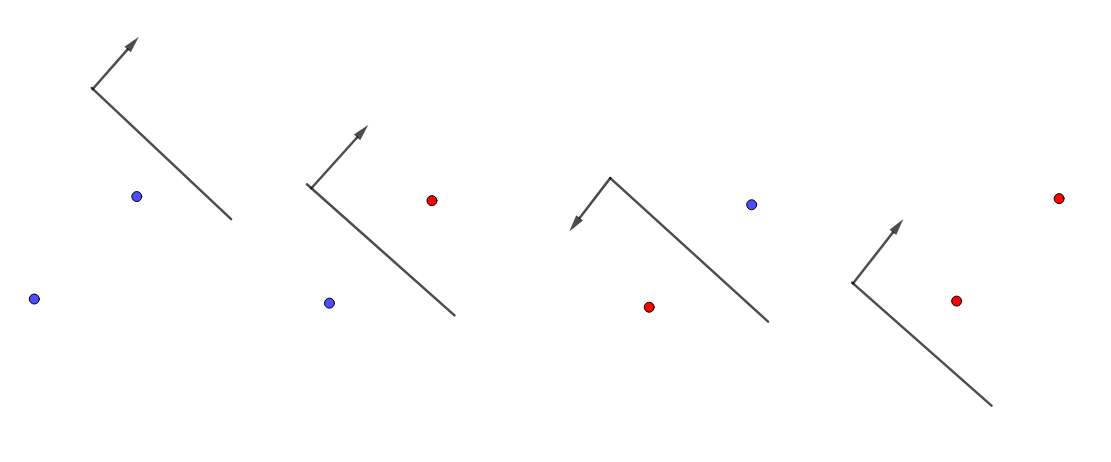
\includegraphics[width=0.75\textwidth]{shattering.png}
\end{center}
Similarly, it is easy to check that any set of 3 points in general position can be shattered as well. However, no set of 4 points can be shattered, as can be seen in the following two exhaustive
cases for points in general position (degenerate cases with more than two points on a line are handled similarly).
\begin{center}
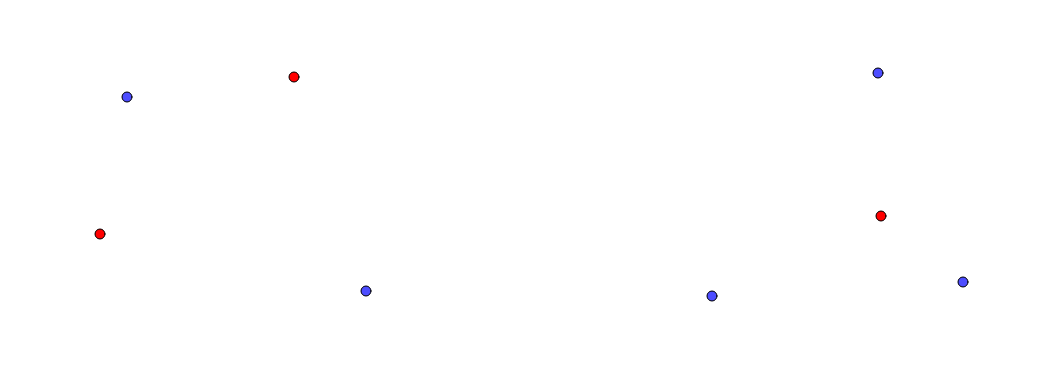
\includegraphics[width=0.75\textwidth]{impossible-shattering.png}
\end{center}
\end{example}
Now that we have an understanding of shattering, we can define the VC dimension of a  hypothesis space $\mathcal{F}$.
\begin{definition}
    The \emph{VC dimension} of a hypothesis space $\mathcal{F}$ is the largest size of a set of points that can be shattered by a member of $\mathcal{F}$.
\end{definition}
\begin{example}
    In the previous example, the VC dimension of $\mathcal{F}$ is $3$, since there is a set of 3 points which can be shattered by $\mathcal{F}$, and no set of 4 points can be shattered by
    $\mathcal{F}$.
\end{example}
\begin{remark}
    It can be shown that the VC dimension of hyperplane classifiers in $n$ dimensions is $n + 1$.
\end{remark}
\begin{remark}
    Hyperplanes have been studied extensively in the context of model complexity, and the reason is that they are some of the simplest constructs, and they have properties that make them
    mathematically tractable and amenable to analysis. It also turns out that due to the kernel trick, and the fact that in a sufficiently high dimensional space, all problems are linearly separable,
    we can work with hyperplanes and still retain a large amount of generality while working with them.
\end{remark}
Note that in this definition, it is not necessary that we should be able to shatter \emph{all} possible sets of size $\text{VC}(\mathcal{F})$; it is sufficient to have at least one possible set of
this size. However, to be able to claim that $k$ is equal to $\text{VC}(\mathcal{F})$, the following statements need to be true:
\begin{enumerate}
    \item There is at least one set of $k$ points which can be shattered.
    \item There is no set of $k + 1$ points which can be shattered.
\end{enumerate}
The VC dimension can thus essentially be thought of as a measure of the capacity of a set of functions.\nl
Note that an important question is the following: given a dataset (a set of samples), what is the required model complexity to be able to learn that dataset? The reason why this question is so
important is that answering this would give us more precise data-specific bounds on how complex our model should be, which is something that the VC dimension completely ignores. However, this question
has largely not been answered yet.\nl
In the same context, one aspect of the samples that seems important, but is missing from the idea of the VC dimension, is the relative arrangement of the data points, in the sense that it is
sufficient to exhibit a single arrangement of points which are shattered, whether that arrangement is relevant to our dataset or not.\nl
Another thing that is somehow counterintuitive according to this definition is that there may exist learning machines with one parameter, but infinite VC dimension. Such a learning machine exists
due to the same fact -- we can claim that the VC dimension is at least $k$ if there is at least one set of $k$ points which can be shattered.
\begin{example}
    (due to E. Levin and J.S. Denker) Let $\theta : \mathbb{R} \to \{-1, 1\}$ be defined as $\theta(x) = 1$ iff $x > 0$. Let $\mathcal{F}$ be the family of functions $\{f_\alpha \mid \alpha \in
    \mathbb{R}\}$ where $f_\alpha(x) = \theta(\sin(\alpha x))$. Suppose we are given a positive integer $l$, and we have to choose a set of $l$ points that can be shattered. We pick $x_i =
    10^{-i}$. Suppose the assigned labels are $\{y_i\}_{i = 1}^l$. Consider $\alpha = \pi \cdot \left(1 + \sum_{i = 1}^l \frac{(1 - y_i) \cdot 10^i}{2} \right)$. It is easy to check that
    $f_\alpha(x_i) = y_i$ for all $i$, so the VC dimension of $\mathcal{F}$ is unbounded (or in other words, infinite).\nl
    However, we can also find a set of 4 equidistant points which can't be shattered (for instance, an example where the second point in the natural order is classified into a different class than
    the rest), but that doesn't affect the fact that the VC dimension of this set of functions is infinite.
\end{example}
What does such an example entail? The VC dimension being infinite implies that we can't use the bound involving the growth function to talk about the probability of choosing a bad
classifier.\nl
More on this topic can be read from \cite{burges}.
\newpage
\section{Gap tolerant classifiers and structural risk minimization}

Before we talk about gap tolerant classifiers, we shall talk about structural risk minimization. From all our discussion about VC dimension, it seems that we can avoid overfitting by learning
models that are not too complex. This is why sometimes we incorporate the model complexity in the loss function to be optimized for, for the purposes of model selection. This is called
structural risk minimization.\nl
We will start off with some motivation for gap tolerant classifiers. The VC dimension bounds mentioned above don't take into account any property of the data. Let's suppose the input data is $n$ dimensional. Firstly, note that the extent of usual sample data is not infinite, so there exists a
ball/hypersphere of some radius $R$ in $\mathbb{R}^n$ which contains all the samples. Let $R$ be the radius of the smallest such hypersphere. We want to somehow take this into consideration. Also, it
is hard to account for misclassifications near the decision boundary as well. With these ideas in mind, we define gap tolerant classifiers.
\begin{definition}
    A gap tolerant classifier is an SVM-like classifier characterized by two hyperplanes and a hypersphere, where the points outside the sphere or inside the margin between the two hyperplanes are always
    deemed to be correctly classified.
\end{definition}
An example of such a classifier can be seen below.

\begin{center}
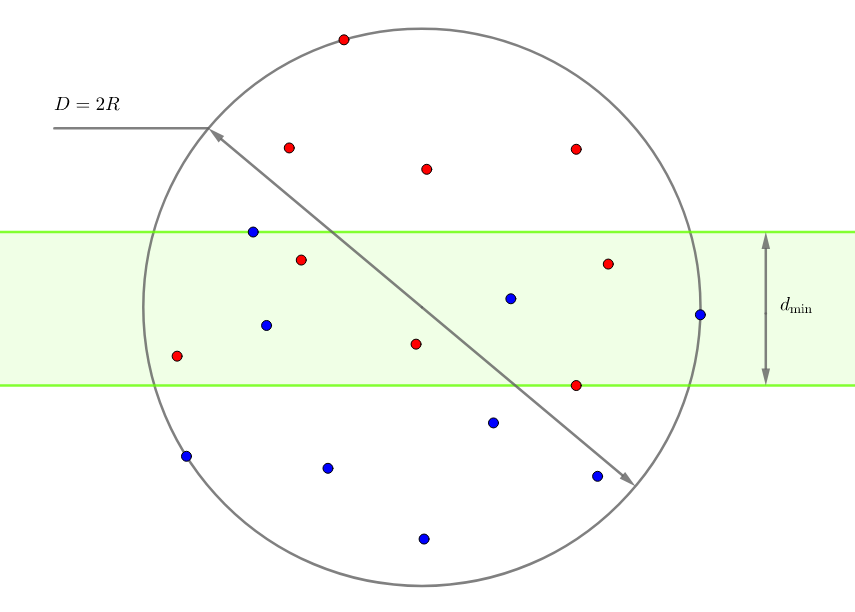
\includegraphics[width=0.75\textwidth]{gap-tolerant-classifier.png}
\end{center}
Points colored red/blue are in class $-1$/$1$ respectively, and we don't care about the classification of points inside the green margin (or outside the hypersphere). All points on one side of the
fat margin should be of a certain class (which is why such classifiers are also called fat-margin classifiers), but the points inside the margin are irrelevant. \cite{burges} notes that for
such classifiers, it is important to use the precise definition of shattering in order to compute the VC dimension (rather than the one used earlier) -- for every possible binary labelling, there is an $f$ that can incorrectly label all
the points (rather than correctly label all points). These classifiers are significant because of the following concrete bound on the VC dimension of this family of classifiers, first
proved by Vapnik in \cite{vapnik2}:

\begin{theorem}
    For a gap-tolerant classifier (for $n$-dimensional data) with the diameter of hypersphere being $D = 2R$ and the width of the margin being $d_{\min}$, the VC dimension is upper bounded by
    $\min\left(\left\lceil\frac{4R^2}{d_{\min}^2}\right\rceil,
        n\right) + 1$.
\end{theorem}
For a given dataset, as mentioned earlier, we can use a gap-tolerant classifier with the hypersphere being the smallest hypersphere that can contain all the points in order to minimize this
bound, while keeping $d$ constant. Note that we don't want $d_{\min}$ to be too large, else it would make our model crude (since we would ignore too many input samples), and we don't want
it to be too small either, else we would not get an appreciable reduction in the VC dimension. What we are doing here is an instance of structural risk minimization, since we are directly trying
to minimize the bound on the VC dimension, which is a measure of model complexity.\nl
Let's look at what happens in the special case when the data is linearly separable. For some given data, the value of $R$ is constant, so the problem reduces to minimizing
$\frac{1}{d_{\min}^2}$. When the data is linearly separable, and we wish to learn a classifier which doesn't have any misclassifications, we have $d_{\min} = \frac{2}{||w||}$ (the
distance from the hyperplane to the closest sample) for a given
hyperplane classifier $w^\intercal x + b$. So the problem reduces to maximizing the margin, which is essentially an SVM. However, there is a problem with this. An argument against this is
that when we apply some transformation to the data, for instance, scaling, then both the $R$ and $d_{\min}$ (as well as $\frac{R^2}{d_{\min}^2}$) change in non-linear ways, which will in turn affect
the bound on the VC dimension (which we will call the radius-margin bound).
This is in fact well-known and corroborates the fact that pre-processing of data in ways like normalization can be helpful for SVMs. There has been work on finding similar bounds for deep
neural networks as well, for instance \cite{sharma}, showing that this idea is not just specific to a certain kind of machine learning models.\nl
Coming back from the digression, this means that we need to do something that is more robust against such changes. As we will see later on, minimal complexity machines are models which minimize
a function of some affine functions of the input samples as an drop-in replacement for the $\frac{R^2}{d_{\min}^2}$ bound, which makes them resistant to scaling. Just like SVMs, they have their
own soft-margin and kernel versions which perform quite well (and have better VC dimension/generalization properties in general, compared to their SVM counterparts). For more information, please refer to \cite{jayadeva}.

\newpage
	\bibliographystyle{plain}
	\begin{thebibliography}{10}
		\bibitem{vapnik}
        Vapnik, V.N., 1999. An overview of statistical learning theory. \emph{IEEE transactions on neural networks, 10}(5), pp.988-999.
		\bibitem{vapnik2}
        Vapnik, V.N., 1998. Statistical Learning Theory. \emph{Wiley, New York.}
        \bibitem{burges}
        Burges, C.J., 1998. A tutorial on support vector machines for pattern recognition. \emph{Data mining and knowledge discovery, 2}(2), pp.121-167.
        \bibitem{moore}
        Moore, A.W., 2001. VC-dimension for characterizing classifiers. \emph{Retrieved from} \texttt{https://www.cs.cmu.edu/\textasciitilde./awm/tutorials/vcdim08.pdf} % has certain errors
        \bibitem{jayadeva}
        Jayadeva, 2015. Learning a hyperplane classifier by minimizing an exact bound on the VC dimension. \emph{Neurocomputing, 149}, pp.683-689.
        \bibitem{sharma}
        Sharma, M. and Soman, S., 2018. Radius-margin bounds for deep neural networks. \emph{arXiv preprint arXiv:1811.01171.}
	\end{thebibliography}
\end{document}
